\chapter{DMC/HiST Systems Operations Guide}
\label{chapter:ops}
\thispagestyle{myheadings}

\graphicspath{{Ops/}}

\section{Summary}
The vision for the DMC and HiST system software and hardware was collaborative and one that would be reusable by its general nature.
By breaking the software and hardware build tasks up into incremental small parts, several engineering undergraduate and graduate students contributed meaningfully in a scaled-down version of the CubeSat teaming model. 
The DMC system is designed as a testbed for HiST multi-site operations, while DMC synchronizes multiple cameras at one site.
The cameras used for DMC were an Andor Neo and Andor iXon, as these were the cameras available at the time and low budget precluded purchasing purpose-obtained cameras.
The Andor Neo sensor coupled with the Marshall \unit[140]{mm} lens gave more resolution than necessary, so 4x4 or 8x8 binning was typically implemented (see section~\ref{sec:dmc} for details).
Cropping and binning the Neo sensor (reduced resolution) leads to a system where the Neo can be used to record all night and post-process (remove unwanted frames) with open-source software tools during the day. 


\section{Experimental Notes}
The DMC system was first controlled remotely on 2012 AUG 29. 
Both cameras were focused at nautical twilight the partly cloudy evening of 2012 AUG 30. 
The Kowa \unit[8.5]{mm} lens was resolving stars to single pixels on the iXon at the edges of the lens--the center focus is not as good. 
The Marshall/Neo focus was bad, and ultimately required removing the dome and replacing with flat glass due to near-field effects with the Marshall large aperture. 
A model of solar zenith angle was implemented to predict when useful observation times would occur, as seen in Figure~\ref{fig:solar2012}. 
\begin{sidewaysfigure}\centering
	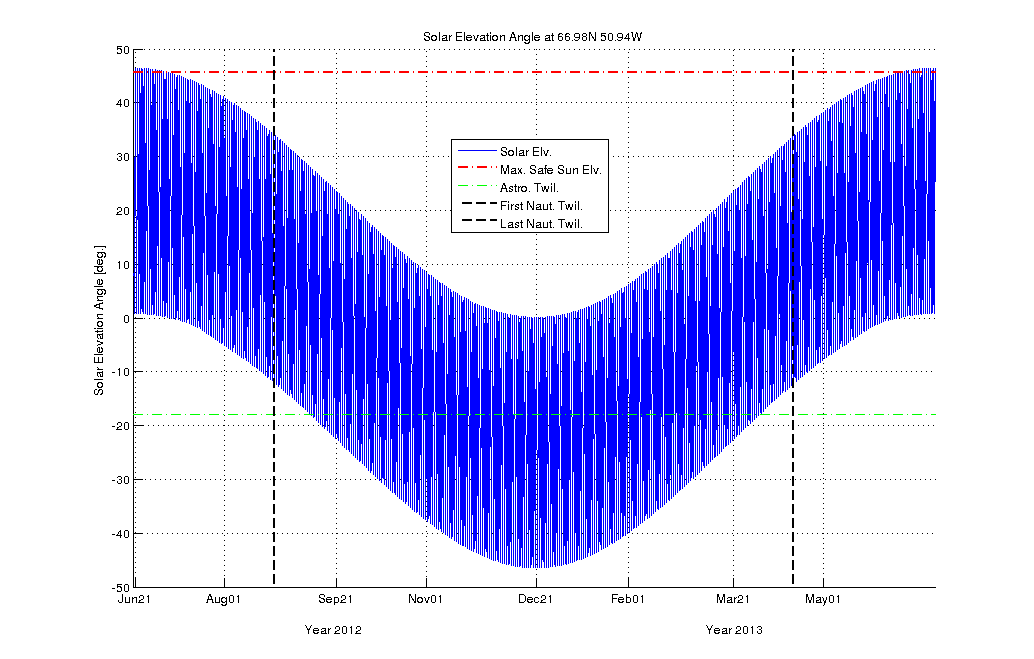
\includegraphics[width=\textwidth]{gfx/Solar2012}
	\caption{Solar elevation at Søndrestrøm}\label{fig:solar2012}
\end{sidewaysfigure}
September through April will provide adequate viewing conditions at night, and the sun is not directly illuminating the sensor during the day.
The plate scaling occurs through \citet{hirschastro,lang2010} for each camera.

Observations on system operation with regard to slow network connection (as occurs due to Greenland Internet or anywhere with weak 3G/4G signal):
\begin{enumerate}
    \item Internet bandwidth is restricted--range of \unit[5]{kB/s} (1996 dialup modem speed) to \unit[60]{kB/s} (3G mobile connection). 
    \item GUI-based remote control is jumpy and sporadic 
    \item Image preview operation are quite slow and rapid progressions of image displays (i.e. video) cause loss of ability to control DMC PC.
    \item Downloads/uploads are dropped repeatedly if bigger than \unit[5]{MB}--files bigger than \unit[5]{MB} must be broken up into multiple segments
    \item lossy 200:1 compression needed to get even simple image previews 
    \item MATLAB campus license does not work due to inaccessible license server off-campus.
\end{enumerate}

Programming software and utilities available on DMC/HiST include: Labview 64-bit, Python 3.6, ImageMagick, Cygwin and Windows Subsystem for Linux.
At the project kickoff, it was decided to start with Labview control as Labview is known for robust multi-threaded control of unattended industrial equipment.
A simple program was written in Labview to start/stop acquisition based on a daily schedule oriented around when SZA$> 100^\circ$.
The Python asynchronous daemon waits for the Labview acquisition to stop, then begins automated computer vision processing of the day's data.
Windows Subsystem for Linux (WSL) is a Microsoft factory feature of Windows allowing access to a very large subset of Linux functionality at nearly the same performance as a bare-metal Linux install from within Windows.
WSL avoids the recompilation hassles and significant performance limitations of Cygwin.
WSL currently comes standard with Ubuntu 16.04 (the latest stable version), and other version of Linux can be installed within WSL as desired.

\section{Automatic Software Workflow}\label{sec:autoAlgo}
\texttt{cron} jobs act as backups to the main Python and Labview daemons, to help protect the cameras in case of an unexpected software failure.
The main Labview program is stored under \texttt{c:/code/lvsite}. 
The basic Labview user interface mirrors the variables stored in XML, so that external programs easily parse the experiment configuration for off-line data use.
Unlike standard Labview programs, the graphical interface is deemphasized because of the slow and intermittent Internet connectivity typical of remote systems.
Each day, four files are saved under folder \texttt{d:/YYYY-MM-DD/} that are automatically read by data post-processing programs.
\begin{table}\centering
    \caption{Files produced each night by the HiST recording software.}\label{tab:filewritten}
    \begin{tabular}{p{2cm}p{12cm}}
    \toprule
    file & description \\
    \midrule
    \texttt{.xml} & Human-readable header file detailing many camera parameters \\
    \texttt{.data} & If cameras had one or more trigger events, this file holds raw 16-bit unsigned grayscale data. May be up to about \unit[400]{GB} in size from a single nights recording, if the iXon recorded all night full-frame at \unit[33]{fps}. Ideally the iXon would trigger only a small portion of the night, recording \unit[17.5]{MB/s} of data \\
    \texttt{.log} & Copies the ``program status'' text box output from the GUI to a file, posts to Dropbox automatically each day\\
    \texttt{.synoptic} & Regardless of trigger status, system records a 16-bit grayscale frame to disk every $N$ Consumer Loop iterations. Typically $N=60$. \\
    \bottomrule
    \end{tabular}
\end{table}

\section{Experiment Design}\label{sec:ExpDes}
The field of view accessible via camera is strongly dependent on frame rate. 
Table~\ref{tab:camParamSpeed} lists a few of the relevant parameters. 
Figure~\ref{fig:ixonFOV} shows the iXon classic projected FOV with frame transfer. 
Figure~\ref{fig:neoFOV} shows the Neo projected FOV with 16-bit readout and global shutter.
Table~\ref{tab:compFPS} shows compatible frame rates between the Neo and iXon with these settings.

Note: FOVs of Figure~\ref{fig:overviewFOV} are notional only with 8.5mm Kowa lens on iXon and 140mm Marshall lens on Neo--actual FOV must be calculated using the desired lens.
\begin{table}\centering
\caption{Compatible frame rates for Neo (16-bit, global shutter) and iXon (14-bit, frame transfer)}
\label{tab:compFPS}
\begin{tabular}{ccc}
\toprule
Frames/sec & iXon (pixels, binning,exp.(ms)) & Neo (pixels,exp.(ms)) \\
\midrule
32.78 & 512 x 512, 1x1, 29.6 & 2560 x 1200, 20.0 \\
61 & 512 x 256, 1x1, 15.1 & 2560 x 600, 12.5 \\
75 & 512 x 206, 1x1, 12.4 & 2560 x 512, 10.5 \\
100 & 512 x 146, 1x1, 9.0 & 2560 x 384, 8.0 \\
\bottomrule
\end{tabular}

\end{table}

\begin{table}\centering
\caption{Camera parameters vs. frame rate effect}
\label{tab:camParamSpeed}
    \begin{tabular}{cccc}
        \toprule
        Camera & Binning & Width & Height\\
        \midrule
        Neo & No & No & Yes\\
        iXon & Yes & No & Yes\\
        \bottomrule
    \end{tabular}
\end{table}
\begin{figure}    \centering
    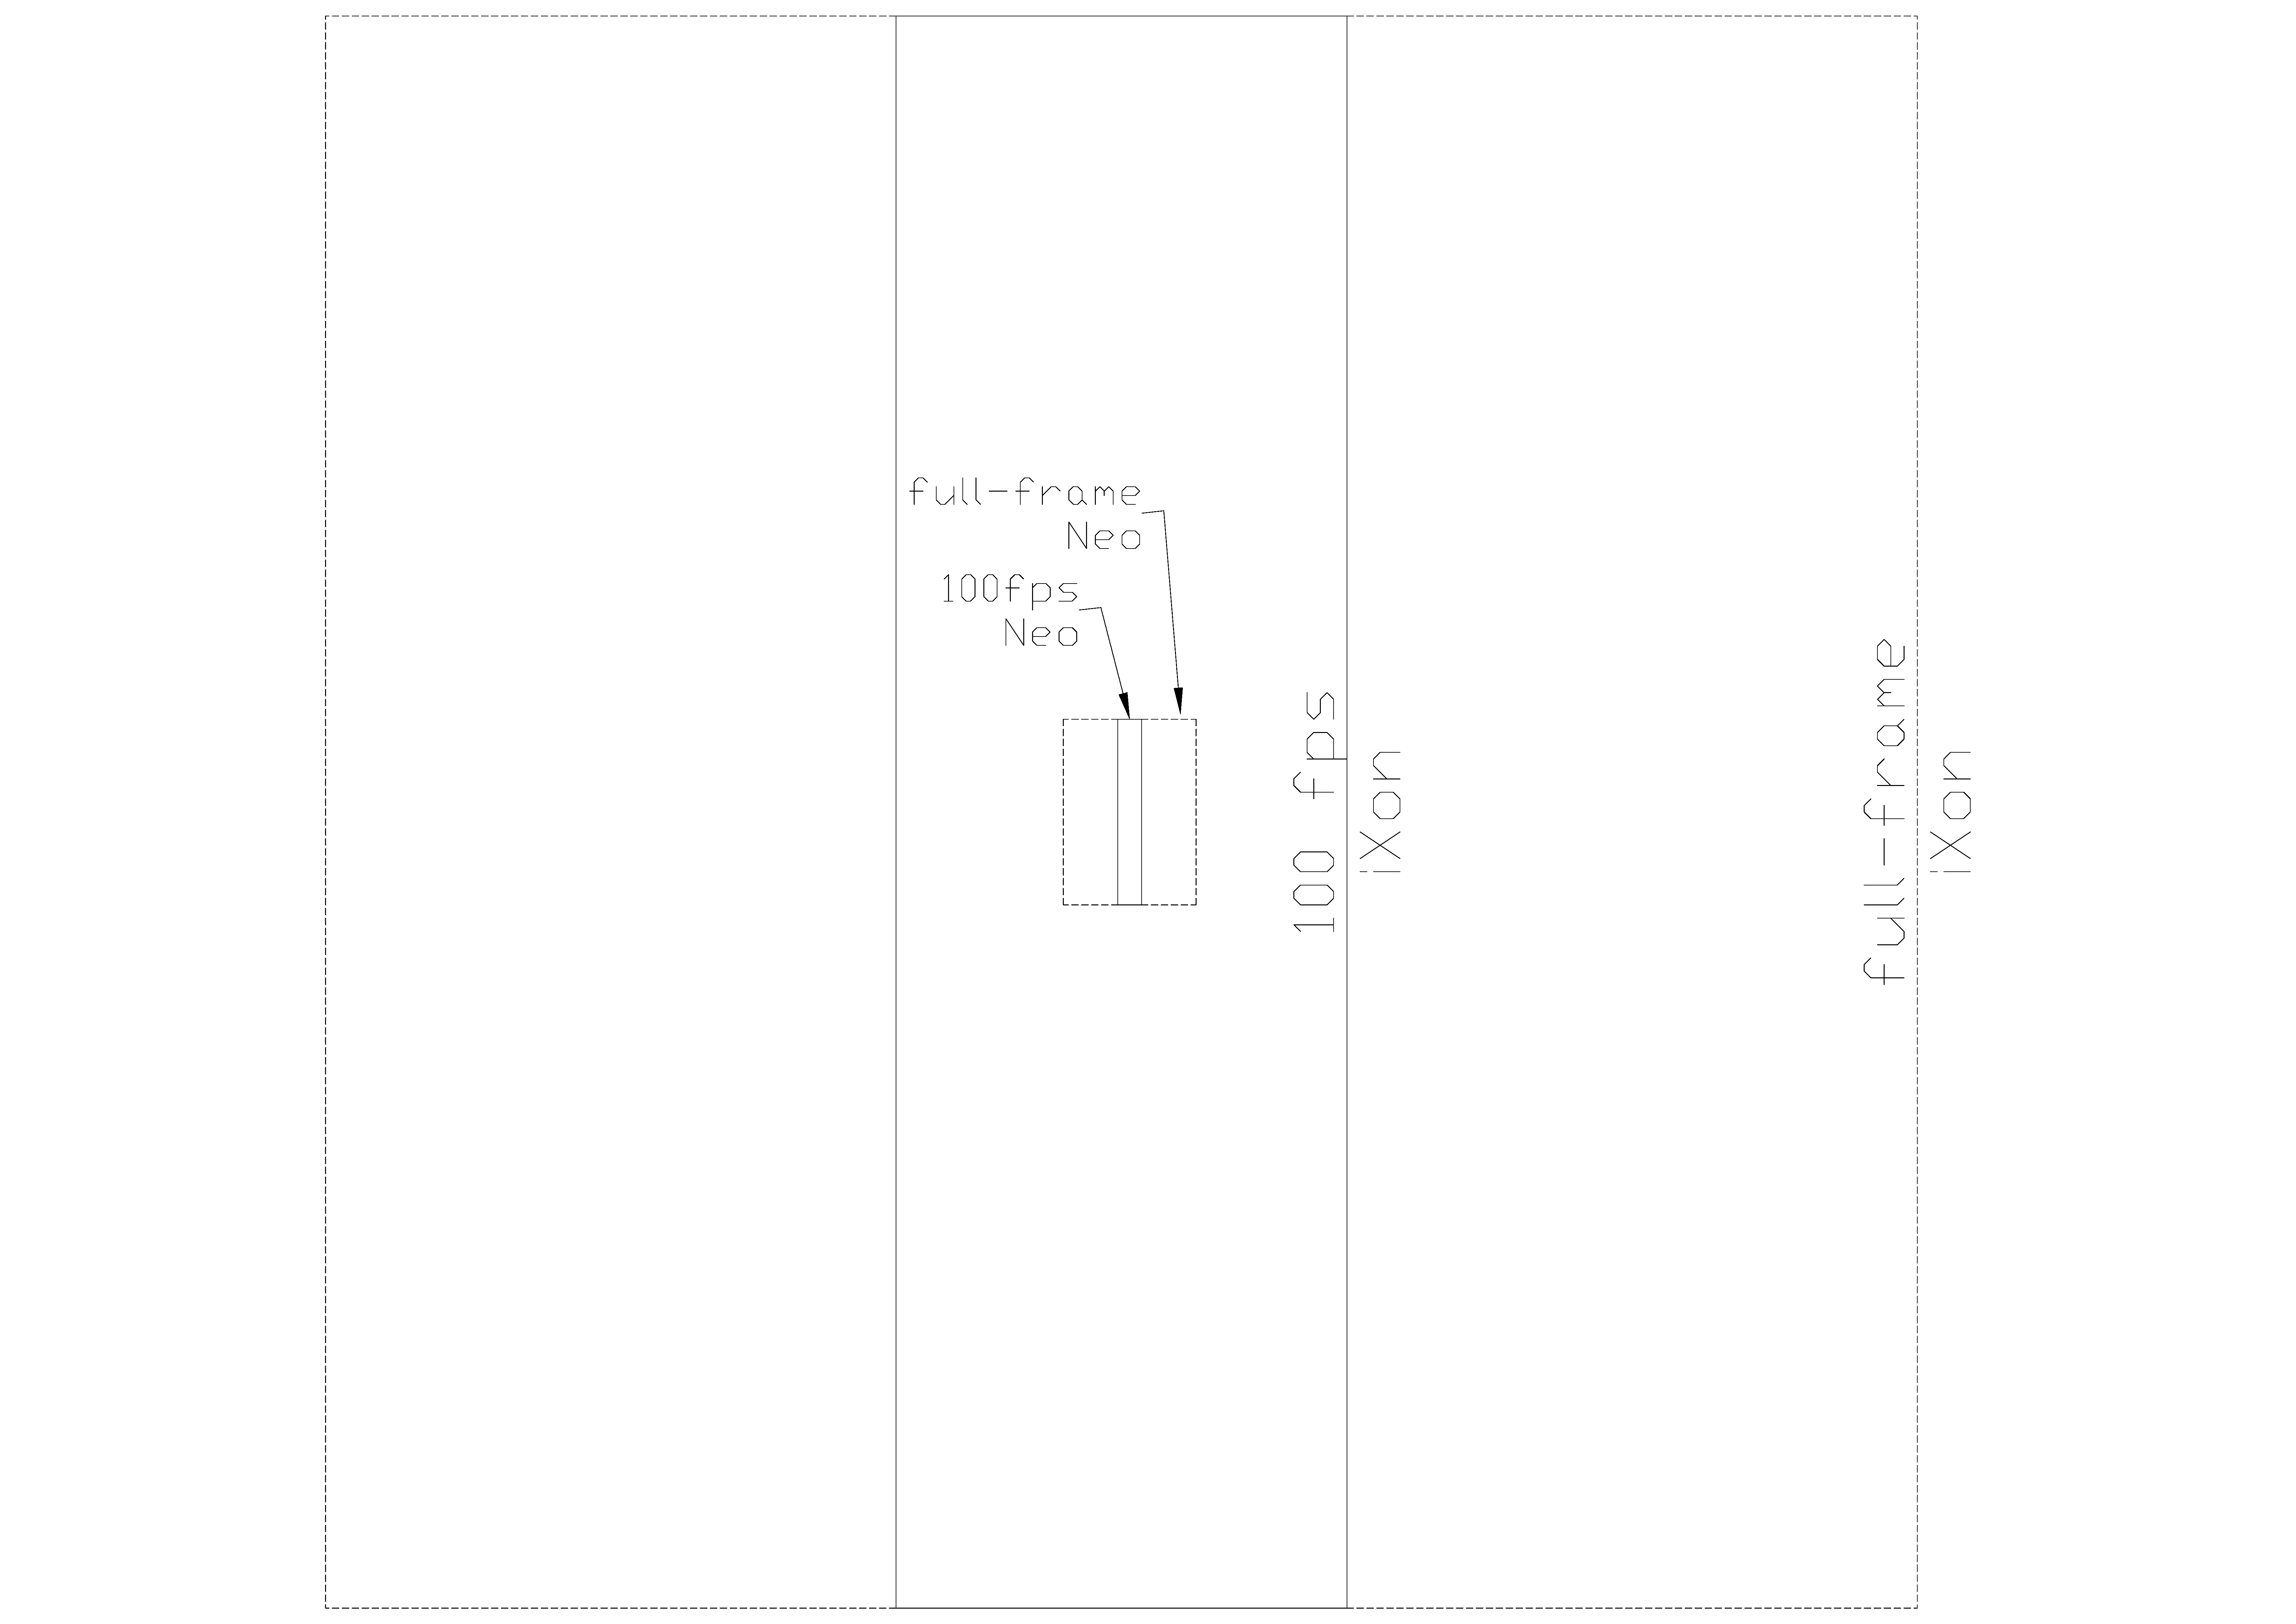
\includegraphics[trim=300 10 300 10,clip,width=\textwidth]{gfx/FOV}
    \caption{Relative FOV of Neo and iXon}\label{fig:overviewFOV}
\end{figure}
\begin{figure}    \centering
    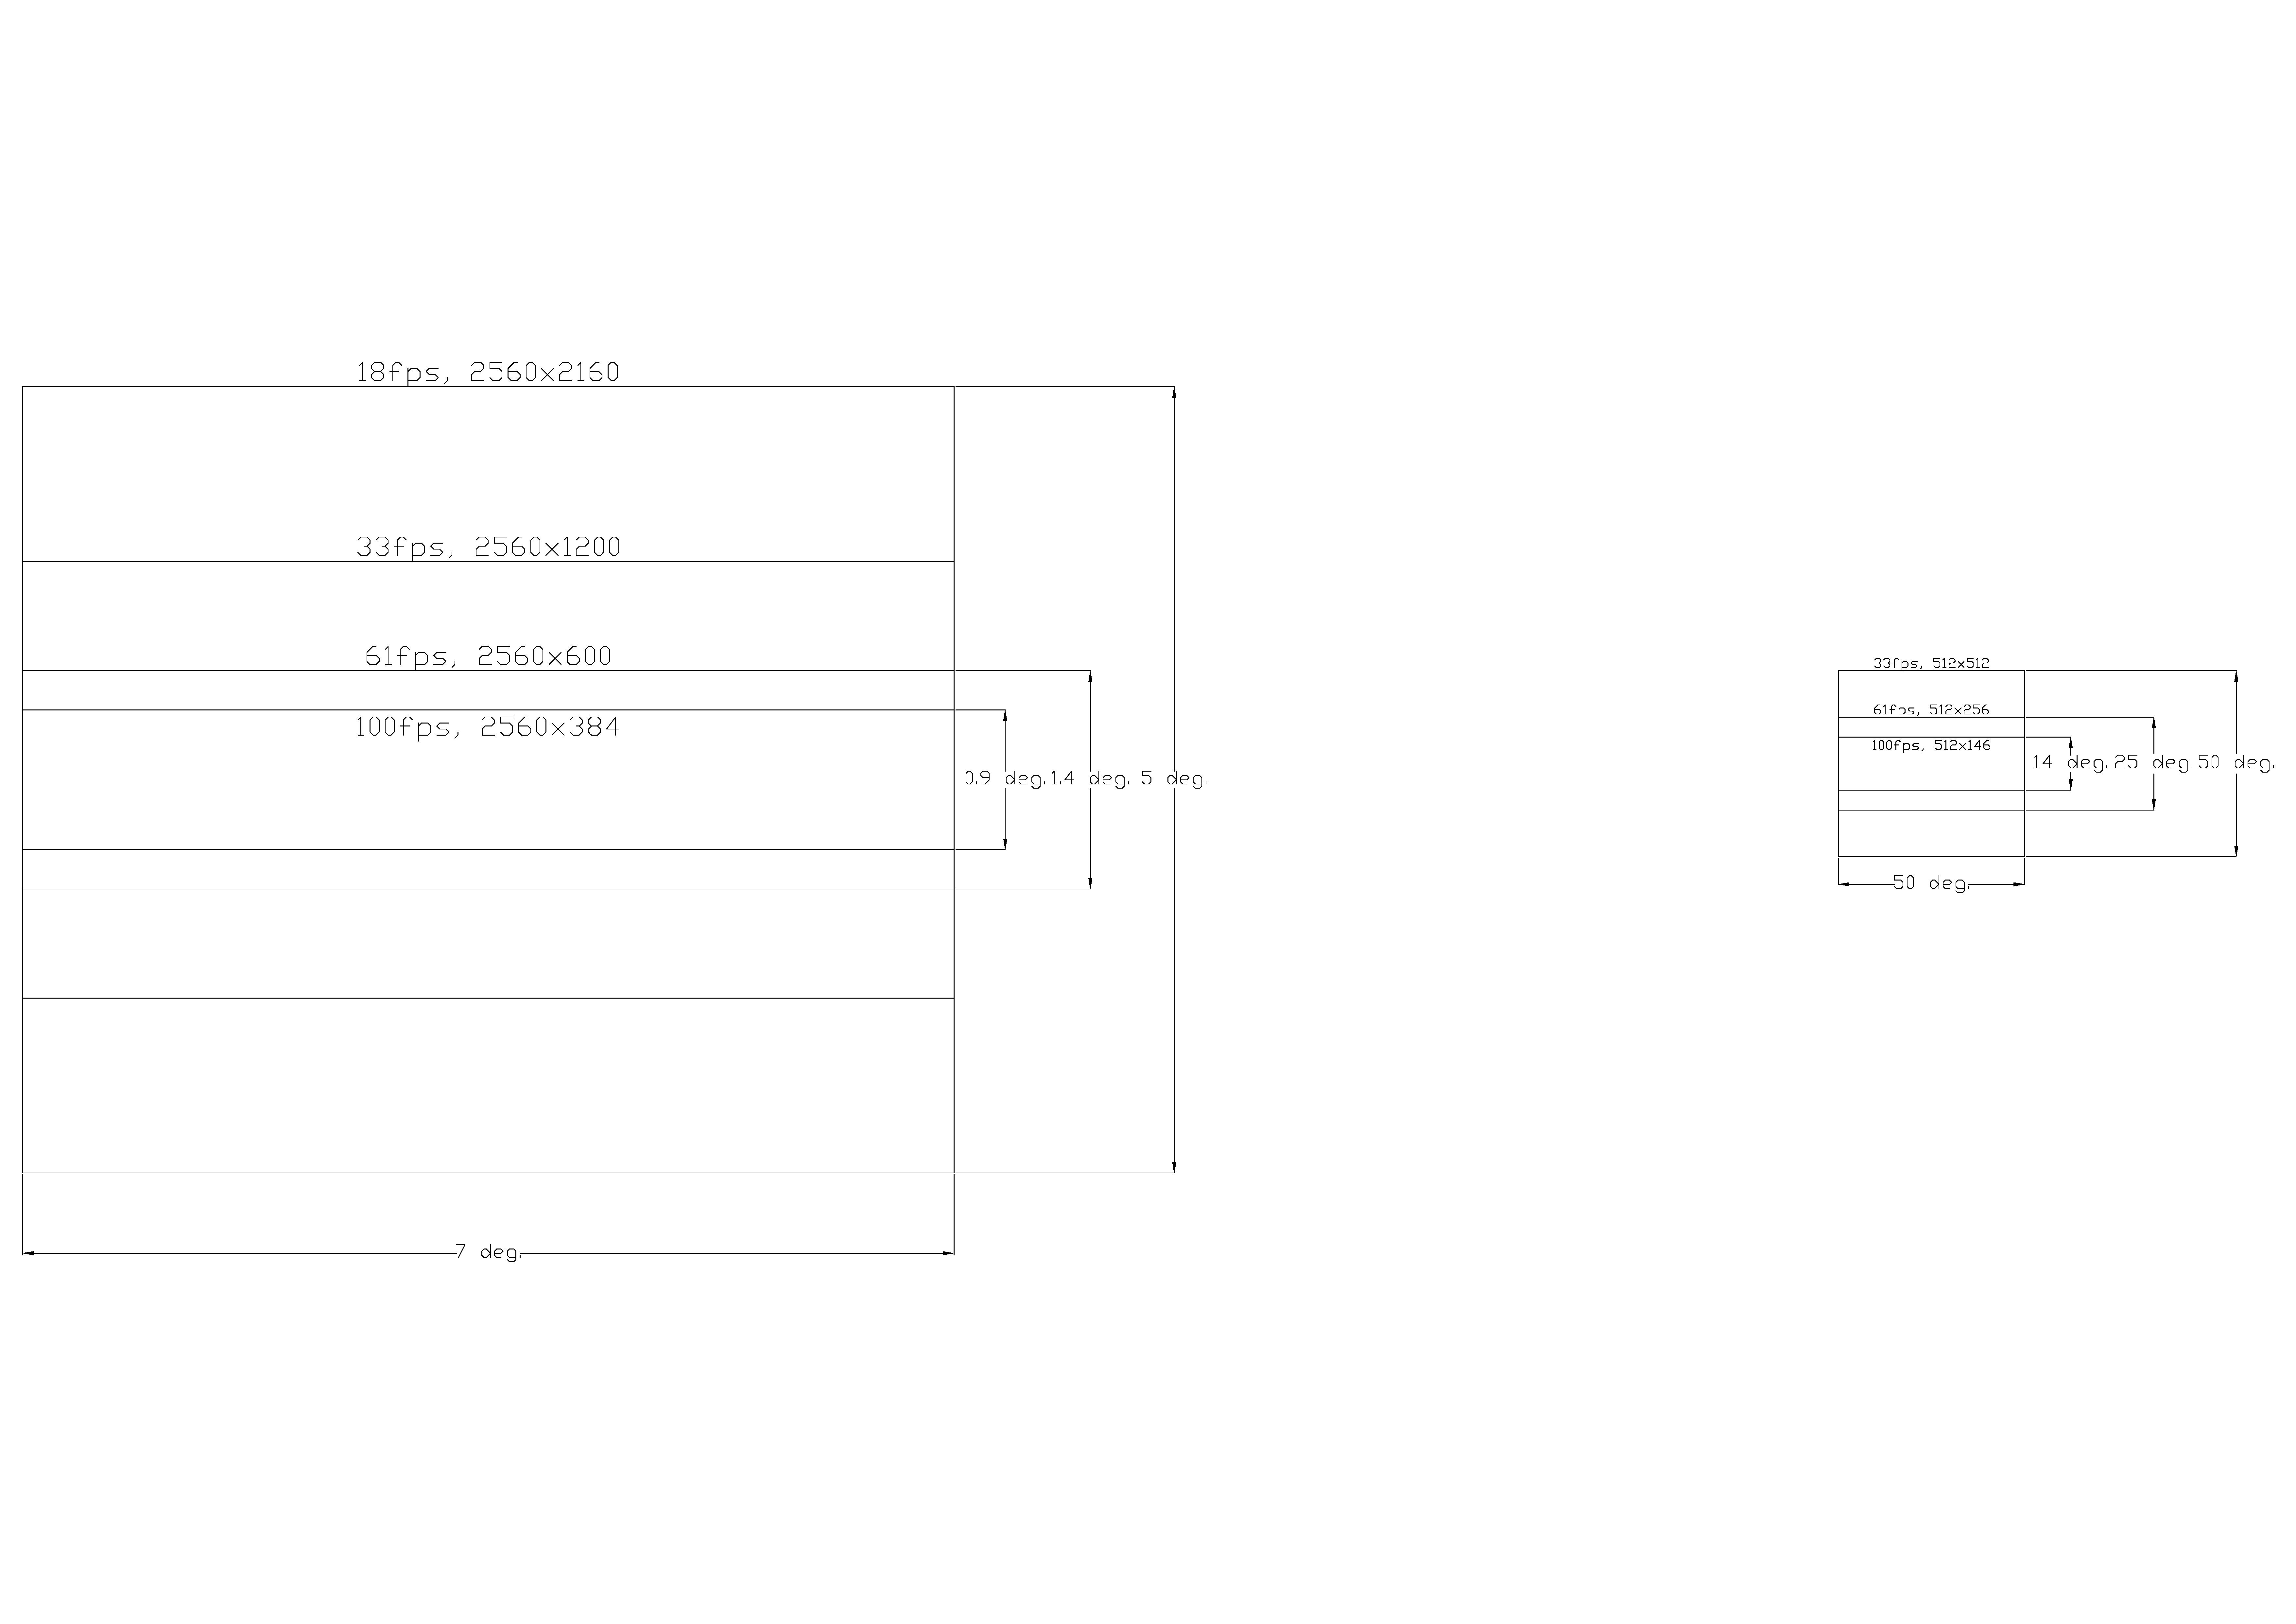
\includegraphics[trim=2650 1050 20 950,clip,width=0.8\textwidth]{gfx/sensorsSize}
    \caption{Notional FOV of iXon with 8.5mm Kowa lens}\label{fig:ixonFOV}
\end{figure}
\begin{figure}  \centering
    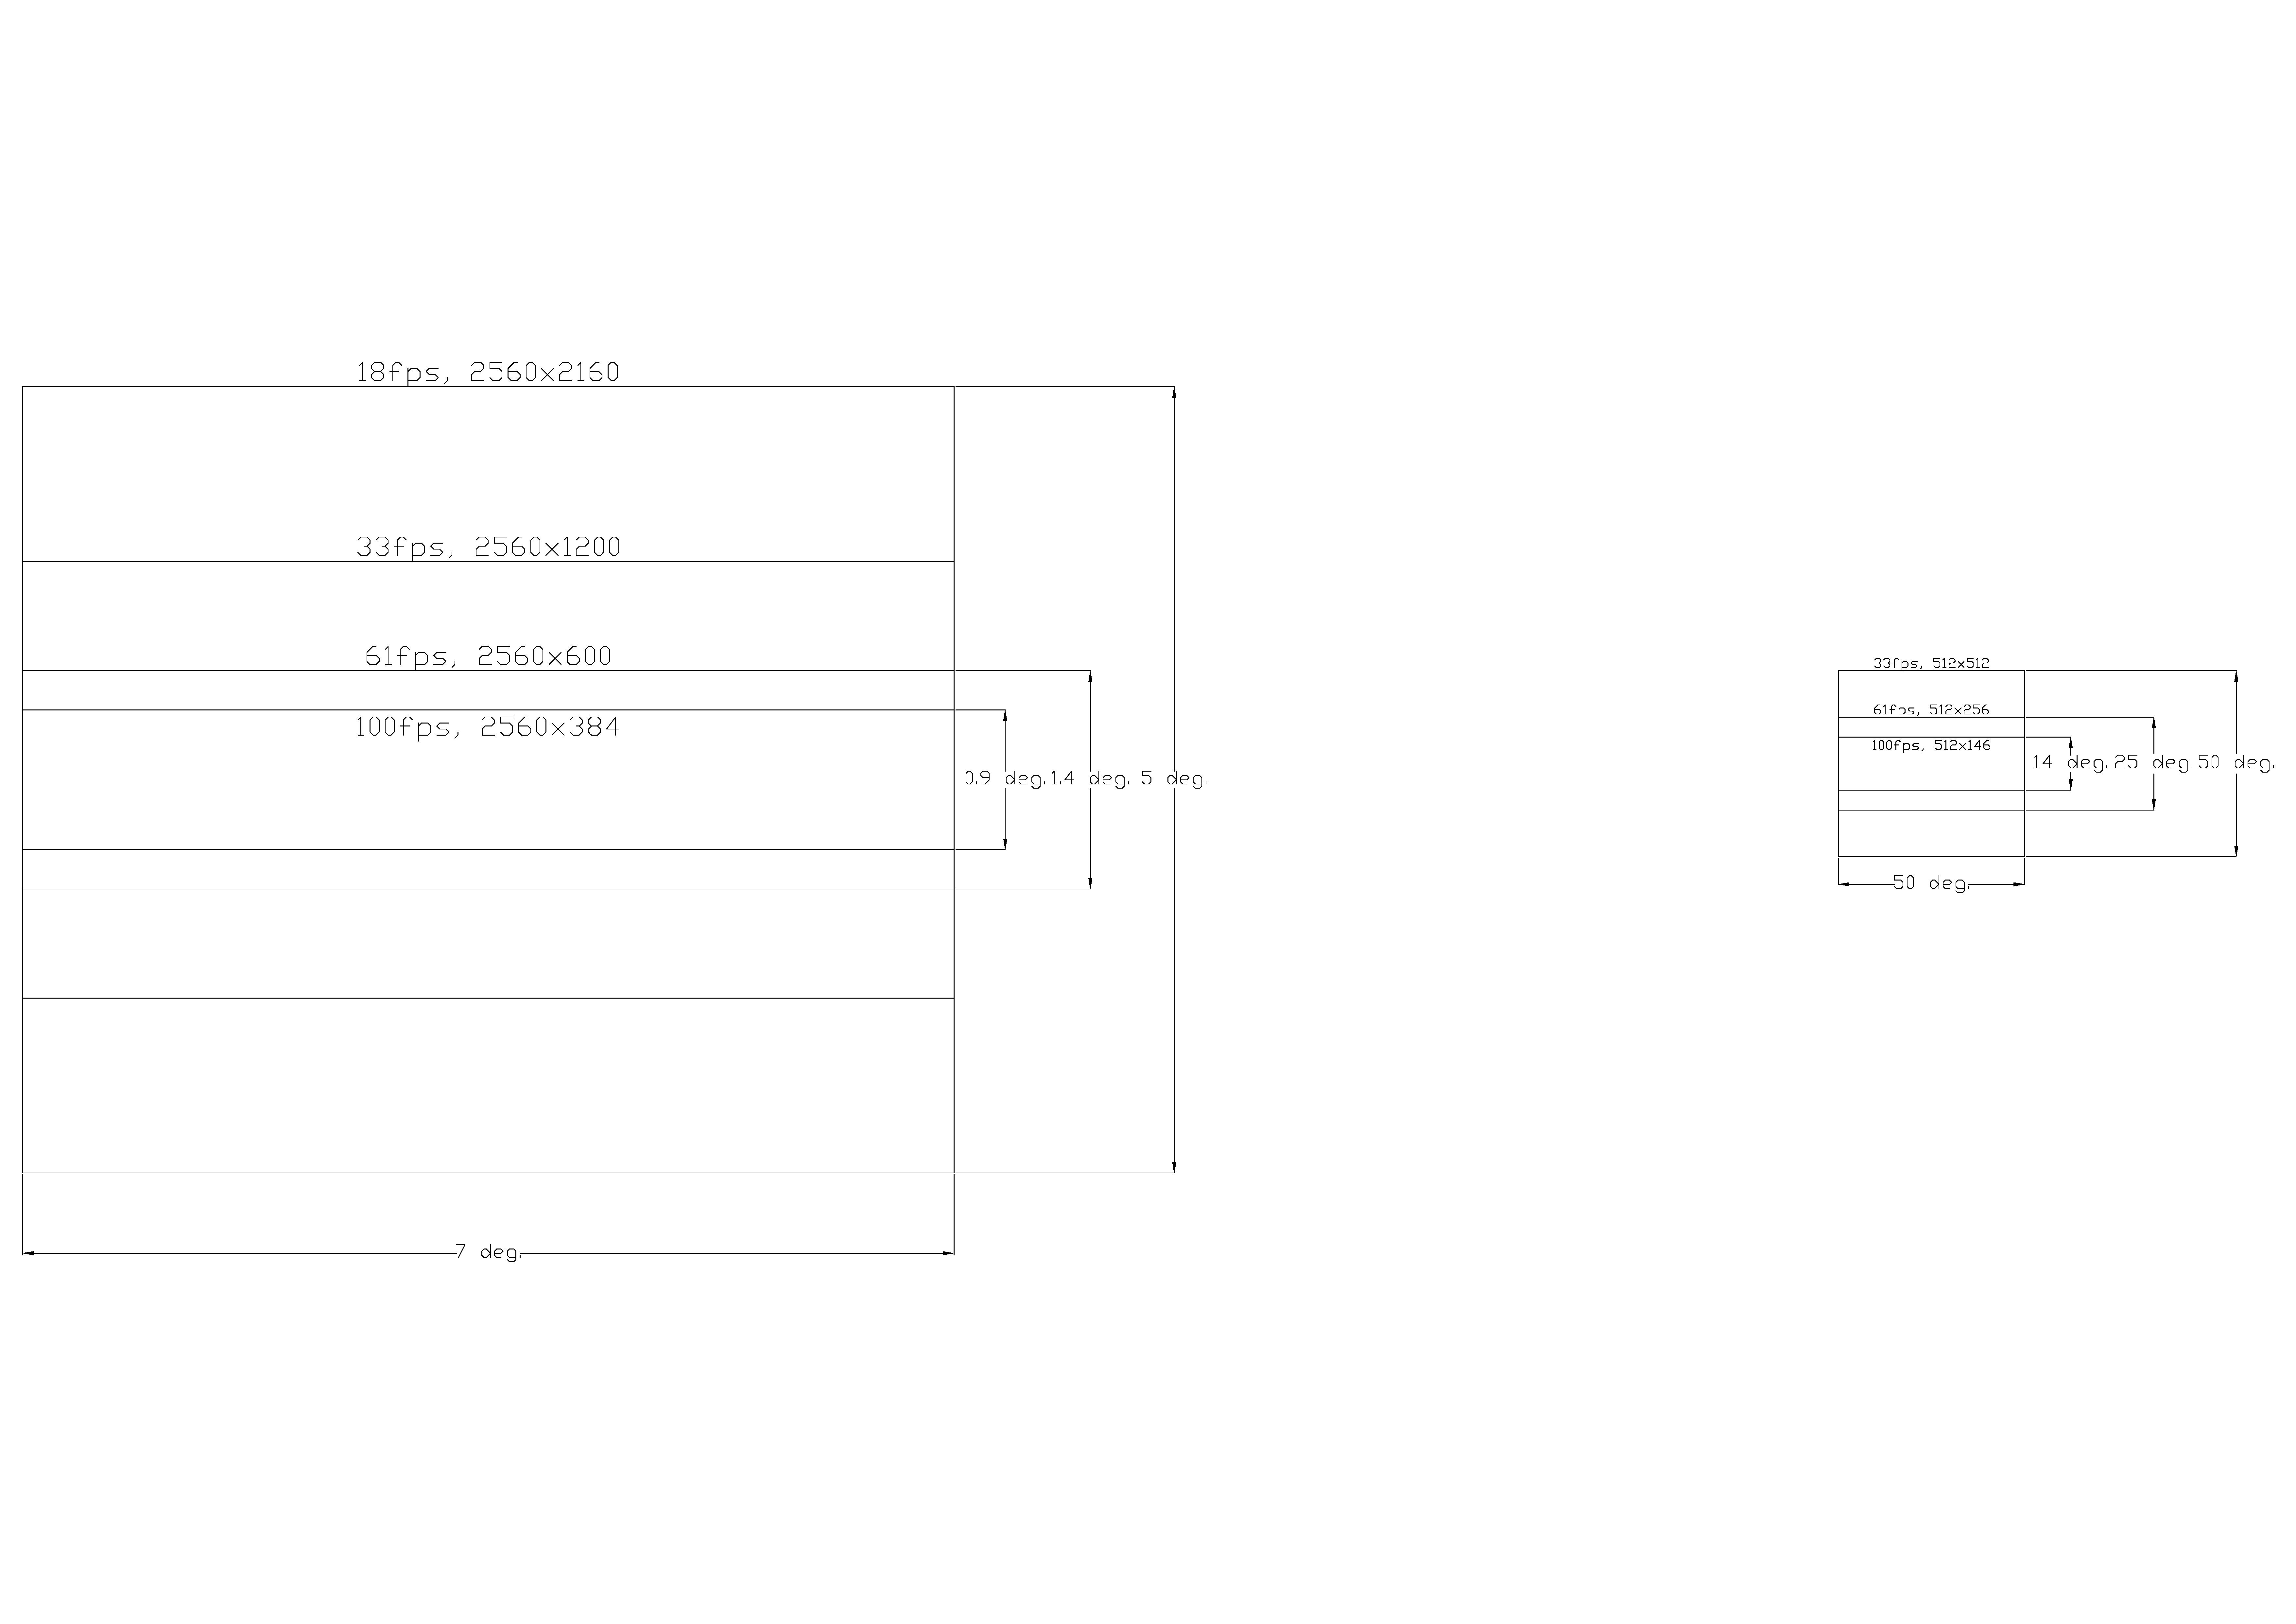
\includegraphics[trim=30 450 1600 450,clip,width=\textwidth]{gfx/sensorsSize}
    \caption{Notional FOV of Neo with 8.5mm Kowa lens}\label{fig:neoFOV}
\end{figure}

\section{LabVIEW data acquisition algorithm}
The Labview algorithm consists of four loops executing in parallel, each with selectable priority. 
This ability is one of the two key reasons Labview was chosen for this project.
The other key reason is that all essential functionality was demonstrated from scratch in two weeks from a blank sheet. 

\subsection*{Producer}

This loop is particular to the camera or device in use--one loop per imaging device.

\begin{algorithm}
	\caption{Producer}
	\begin{algorithmic}
		\While{SZA $> 100^\circ$}
		\If{numberOfFramesInBuffer $> M$}
			\State  PCIe FPGA $\leftarrow$ $M$ frames $\leftarrow$ Camera FPGA 
			\State DMA: PC RAM Ring buffer $\leftarrow$ $M$ frames $\leftarrow$ PCIe FPGA
		\EndIf
		\EndWhile
	\end{algorithmic}
\end{algorithm}

\subsection*{Consumer}
This loop is generic--one loop per imaging device.

\begin{algorithm}
	\caption{Consumer}
	\begin{algorithmic}
		\Procedure{Long term storage}{}
		\While{SZA $> 100^\circ$}
		\State HDD $\leftarrow$ RAM Queue
		\EndWhile
		\EndProcedure

		\Procedure{Synoptic Recording}{}
		\While{SZA $> 100^\circ$}
			\If{more than $N$ seconds since last synoptic frame}
			\State HDD \texttt{.synoptic} file $\leftarrow$ average image of last ten frames in Queue
			\State Copy last frame of synoptic file to \texttt{.png} for web server ``live'' image
			\EndIf
		\EndWhile
		\EndProcedure
	\end{algorithmic}
\end{algorithm}

\subsection*{Network}
This loop handles orderly shutdown of the system from error or remote commands.
It uses TCP/IP sockets implemented as Labview Network Shared Variables to accomplish this.

The ``SanityCheck'' range of expected intensities $I$ is based on a 16-bit camera--adjust according to the relevant device.
Here, 100 is chosen as a number below the mean imaging chip noise based on typical camera gain settings.
For a narrow FOV camera with BG3 filtering, the image should never saturate with diffuse aurora. 
Saturation (low or high values) may be an indication of excess light reaching the imaging chip, therefore the system shuts down for the night, which closes the built-in camera shutter.
An example of a situation outside of system failure that might introduce excess light is a flashlight or laser shining into the camera--recall these cameras are deployed to unattended locations where anyone might walk by.

\begin{algorithm}
	\caption{Network}
	\begin{algorithmic}
		\Procedure{Failsafe}{}
		\While{SZA $> 100^\circ$}
		\State Poll TCP/IP socket values
		\If{NetworkShutdown \textbf{or} Error}
		\State Stop Producer and Consumer loops
		\EndIf
		\EndWhile
		\EndProcedure
		
		\Procedure{SanityCheck}{}
		\While{SZA $> 100^\circ$}
		\If{last three \texttt{.synoptic} $100 < \overline{I} < 60000 $ }
		\State Stop Producer and Consumer loops as saturation may be indication of excess light on imager chip
		\EndIf
		\EndWhile
		\EndProcedure
	\end{algorithmic}
\end{algorithm}

\subsection*{Schedule}
The schedule loop is the outermost loop, never closing except by operator command.
It starts and stops the recordings each day.
\begin{algorithm}
	\caption{Schedule}
	\begin{algorithmic}
		\Repeat
		\If{SZA $> 100^\circ$}
		\State Start Producer, Consumer, and Network loops
		\EndIf
		\If{SZA $< 100^\circ$}
		\State Stop Producer and Consumer loops
		\EndIf
		\Until{Operator Shutdown}
	\end{algorithmic}
\end{algorithm}

\section{Manual Software Workflow}\label{sec:ManWork}
This section covers diagnostic functions that are generalizable to auroral imaging systems.
The software that controls day-to-day recording should generally not have a graphical output for best overall system stability.
This allows the software to run without a graphical desktop at all, greatly enhanced operating system stability and security.
This principle greatly simplifies the recording software, further increasing robustness.
The camera is aimed and focused using the Andor Solis software, which also installs the camera SDK.
The operation of the system is automatically verified by basic sanity checks of the \texttt{.synoptic} file in the Network loop.


The operation of the system may be manually verified upon login to the Flask webserver on each site's PC.
This Flask server is not made available to the public to avoid DDOS-style attacks.
However, an external webserver may poll the cameras (with Flask configured to protect against excessive poll rates) and relay the latest pictures to the public.
This is implemented at the Søndrestrøm site.


The Python script used for detection of Alfvénic aurora is described in chapter~\ref{chapter:discrim}.
The Alfvénic aurora detection algorithm \citep{cviono} may be manually run by executing the command
\begin{verbatim}
python Detect.py ~/data/YYYY-MM-DD/*.DMCdata -p dmc.ini
\end{verbatim}
where \texttt{YYYY-MM-DD} is according to the data date of interest.

\subsection{Connecting to the DMC/HiST systems}
The systems are securely remotely controlled via SSH Public Key Authentication.
This means authorized users must have an encrypted file pair \textit{and} the corresponding password to access the system.
Each PC used to control the system remotely has a unique key, so that individual users can be deactivated if a problem occurs.
A simple script (saved to a text file) is executed to connect.
\begin{verbatim}
#!/bin/sh
ssh -f -p 22 -L 3391:4.3.2.1:3389 1.2.3.4 sleep 1;
xfreerdp /cert-ignore /v:localhost:3391
\end{verbatim}

